\documentclass[a4paper,12pt]{article}
\usepackage[margin=0.7in]{geometry}
\usepackage[latin1]{inputenc}
\usepackage[english]{babel}
\usepackage{amsmath}
\usepackage{cases}
\usepackage[makeroom]{cancel}
\usepackage{amsmath,tabu}
\usepackage[fleqn]{mathtools}
\usepackage[fleqn]{amsmath}
\usepackage{bm}
\usepackage{tikz}
\usepackage{enumitem}
\usepackage{wrapfig}
\usepackage{graphicx}
\usepackage{siunitx}
\usepackage{microtype}
\usepackage{array,tabularx}
\usepackage{float}
\usepackage{booktabs}
\usepackage{myUnitOfMeasure}
\usepackage{myThermodynamics}
\usepackage{myMath}

\title{\textbf{PRECEPT 4}: Repowering of a cogeneration plant}
\author{Rossi Andrea 875272}
\date{}


%\newcommand{\pointdatatable}[5]{
%\begin{center}
%\tabulinesep=1.2mm
%\begin{tabu}{|l|c|c|c|}
%\hline
%$ T_{#1} $ & $ p_{#1} $ & $ h_{#1} $ & $ s_{#1} $\\ \hline
%$ \round{#2} \celsius $ & $ \round{#3} \,bar $ & $ \round{#4} \kjkg $ & $ \round[round-precision=4]{#5} \kjkgk $\\ \hline
%\end{tabu}
%\end{center}
%}

\renewcommand{\thesubsection}{\thesection.\Alph{subsection}}

%
%
%
%
%
%
%
%
%
%
%
\begin{document}
\maketitle

The aim of this precept is to analyse the feasibility of converting a cogeneration plant equipped with an extraction and condensing steam turbine in a combined cycle, by adding to the existing facility a gas turbine. In the repowering, the boiler and feedwater heaters are replaced by a heat recovery steam generator (HRSG), which supplies steam to the power cycle and to the thermal process connected to the plant. With reference to the attached drawings, this consists of transforming configuration A (actual plant layout) into configuration B. For the two cases, the following performance figures should be compared: the net electrical power of the plant, the total efficiency, the net electrical LHV efficiency, the thermal efficiency, the primary energy savings index allowed by cogeneration. 

\section{Performance of the old power plant (layout A) }
Plant A is a natural gas fired boiler with extraction and condensation and it has the following scheme:

\begin{figure}[h]
  \caption{Layout A.}
  \centering
    \includegraphics[width=\textwidth]{plantA_fig}
\end{figure}

The main performance parameters of a cogeneration power plant are:
\begin{itemize}
\item Electric net efficiency $\displaystyle \eta_{el} = \frac{\Wel}{\Qfuel}$.
\item Thermal net efficiency $\displaystyle \eta_{th} = \frac{\Qth}{\Qfuel}$.
\item Total net efficiency $\displaystyle \eta_{I} = \eta_{el} + \eta_{th} = \frac{\Wel+\Qth}{\Qfuel}$.
\item Primary energy saving $\displaystyle PES = 1-\frac{\Qfuel}{\Wel/\eta^{REF}_{el}  +  \Qth/\eta^{REF}_{th}}$.
\end{itemize}
In cogeneration the most significant is the last one, PES, because it gives an idea on how much energy is saved respect to have two different plant, one that produces energy, one that produces thermal power. If $PES<0$ means that it does not make sense to have a cogeneration intgrated plant respect to two separated plant.

With the two basic thermodynamical properties, $p$ and $T$ in every point of the plant we can evaluate all the missing variables.
\\To evaluate the thermal power generated we make an energy balance around the user:
\begin{align}
\Qth &= \mdoth{IN} - \mdoth{OUT_1} -  \mdoth{OUT_2}\\
	 &= \mdoth[user]{IN} - \mdoth[user1]{OUT} -  \mdoth[user2]{OUT}\\
	 &= \round{83709.8837796313/1000}\mw
\end{align}
\begin{conditions}
h^{user}\IN & $h(198\celsius, 5\,bar) = \round{2851.60179874724}\kjkg$;\\[0.5em]
h^{user1}\OUT & $h(90\celsius, 1\atm) = \round{376.992520542715}\kjkg$;\\[0.5em]
h^{user2}\OUT & $h(15\celsius, 1\atm) = \round{63.0790076386603}\kjkg$;\\[0.5em]
\end{conditions}
To compute the chemical energy of the fuel we can make an energy balance on the boiler and then remembering that $\eta_{boiler} = \dot{Q}_{boiler}/\Qfuel$:
\begin{equation}
\Qfuel = \frac{\dot{Q}_{boiler}}{\eta_{boiler}} = \frac{\mdot{boiler} \cdot \left( h^{boiler}\OUT - h^{boiler}\IN	\right)}{\eta_{boiler}} = \round{241422.24397749/1000}\mw
\end{equation}
\begin{conditions}
h^{boiler}\OUT & $h(538 \celsius, 110 \,bar) = \round{3.482284742023043e+03}\kjkg$;\\[0.5em]
h^{boiler}\IN & $h(243 \celsius, 90 \,bar) = \round{1.052553378652162e+03}\kjkg$;\\[0.5em]
\end{conditions}
Finally with all the power exchanged in the plant we can evaluate all the performance parameters:
\begin{itemize}
\item Electric net efficiency $\displaystyle \eta_{el} = \frac{\Wel}{\Qfuel} = \round{0.268409401438759*100}\perc$.
\item Thermal net efficiency $\displaystyle \eta_{th} = \frac{\Qth}{\Qfuel} = \round{0.346736416663563*100}\perc$.
\item Total net efficiency $\displaystyle \eta_{I} = \eta_{el} + \eta_{th} = \frac{\Wel+\Qth}{\Qfuel} = \round{0.615145818102322*100}\perc$.
\item Primary energy saving $\displaystyle PES = 1-\frac{\Qfuel}{\Wel/\eta^{REF}_{el}  +  \Qth/\eta^{REF}_{th}} = \round{-0.115425716688180}<0$.
\end{itemize}

\section{Performance of the new power plant (layout B) }
Plant B respect to A replaces the boiler with a HRSG (heat recovery steam generator) feeded by a gas turbine with bleaeding to power a heat user and it has the following scheme:

\begin{figure}[h]
  \caption{Layout B.}
  \centering
    \includegraphics[width=\textwidth]{plantB_fig}
\end{figure}

Before to procede we must specify four assumptions:
\begin{enumerate}
\item We keep the same steam turbine so the mass flow coefficient $\phi$ is the same for the two cases.
\item The heat user is the same so we have the same thermodynamical and flow rate conditions at the inlet and at the outlet of the user for the two cases.
\item The heat rejection parameters are the same ($\left.U \cdot A \right|_A = \left.U \cdot A \right|_B$ = constant). 
\item The cooling water, in terms of mass flow rate and inlet temperature, is the same.
\end{enumerate}

\subsection{High pressure section}
In a-b section we have the high pressure steam drum and the high pressure superheater;
\begin{figure}[h]
	\centering
    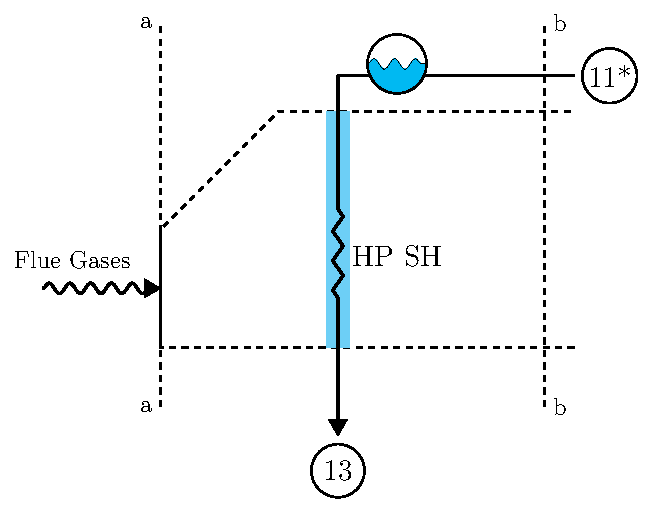
\includegraphics[scale=0.7]{sectionab_fig.pdf}
    \caption{a-b section flows scheme.}
    \label{fig:sectionab}
\end{figure}
From the energy balance in the a-b section of the heat recovery steam generator we get:
\begin{equation}
\mdot{FG} \cdot c_{p_{FG}} \cdot (T_a-T_b) \cdot (1-\xi_{HRSG}) = 
\mdoth{13}-\mdoth{11\first} = \mdot{13} \cdot (h_{13} - h_{11\first})
\label{eq:hp_energy_balance}
\end{equation}
\begin{conditions}
\h{11} & $h(\p{11\first}, \T{11\first})$;\\[0.5em]
\p{11} & evaporation pressure in HP section;\\[0.5em]
\T{11} & $\T{sat}(\p{evap}^{HP})$;\\[0.5em]
\h{13} & $h(\p{13}, \T{13})$;\\[0.5em]
\p{13} & $\p{evap}^{HP} \cdot \left( 1- \left. \frac{\Delta p}{p} \right\rvert_{SH} \right)$;\\[0.5em]
\T{13} & $\T{a}-\Delta\T{\text{pitch point}}$ or at maximum $538 \celsius$;\\[0.5em]
\T{b} & $\T{sat}(\p{evap}^{HP})-\Delta\T{\text{pitch point}}$;\\[0.5em]
\end{conditions}
\begin{figure}[h]
	\centering
    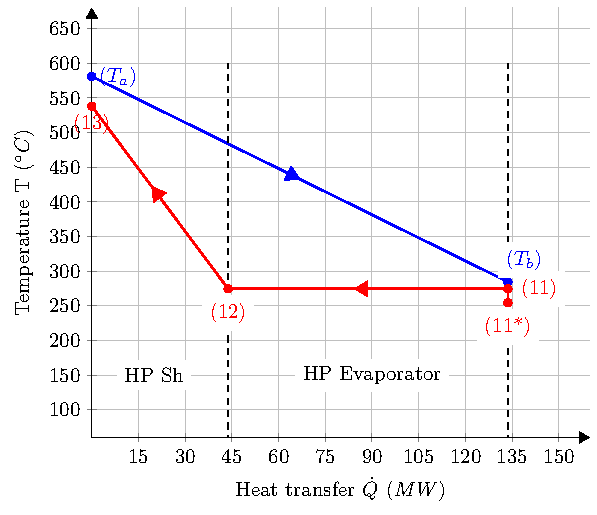
\includegraphics[scale=1]{TQ_plot_HP_fig.pdf}
    \caption{T-Q diagram of a-b section.}
    \label{fig:sectionab_TQ}
\end{figure}
Now we have two unknowns, but just one equation. So we need to use assumprion number 1, that for both layout A and layout B the mass flow coefficient $\phi$ is the same. For case A we know everything so we can easily evaluate $\phi = \mdot{} \cdot \sqrt{T}/p$:
\begin{equation}
\phi_A = \mdot{A}^{\text{turbine inlet}} \cdot \frac{\sqrt{\T{A}^{\text{turbine inlet}}}} {\p{A}^{\text{turbine inlet}}}
= \round{29.556632591069250}
\end{equation}
\begin{conditions}
T & temperature in $k$;\\[0.5em]
\end{conditions}
Reverting the definition of $\phi$ for plant B we can obtain the mass flow rate at the inlet of the high pressure turbine $\mdot{13}$ as a function of the other unknown $p_{evap}$.
\begin{equation}
\phi_B = \mdot{B}^{\text{turbine inlet}} \cdot \frac{\sqrt{\T{B}^{\text{turbine inlet}}}} {\p{B}^{\text{turbine inlet}}} 
= \mdot{13} \cdot \frac{\sqrt{\T{13}}}{\p{13}} = \phi_A
\quad \Rightarrow \quad
\end{equation}
\begin{equation}
\mdot{13} = \phi_A \cdot \frac{\p{13}}{\sqrt{\T{13}}}
= \phi_A \cdot \frac{\p{13}(\p{evap}^{HP})}{\sqrt{\T{13}(\p{evap}^{HP})}}
= f(\p{evap}^{HP});
\end{equation}
Replacing all the relationship we have found in equation \ref{eq:hp_energy_balance} we obtain an equation where the only unknown is $\p{evap}^{HP}$. Due to the non linearity we must solve it with a numeric iterative method. We cannot take the derivative of relations from \md so it is necessary to use a method that does not require first or higher order derivative. So we use secant algorithm and we get that $\p{evap}^{HP} = \round{59.0417409056891}\,bar$. 
Replacing $\p{evap}^{HP}$ in every expression we miss before we obtain that $\mdot{13} = \round{56.983152206110724} \kgs$ and all the thermodynamical properties of points 11 and 13 in table \ref{table:point11_13}.
\begin{table}[h]
\centering
\caption{Thermodynamical properties of points 11 and 13.}
\label{table:point11_13}
\begin{tabular}{@{}lccc@{}}
\toprule
Point & p                               & T                           & h                               \\ \midrule
11$\first$    & $\round{59.041740905689}\,bar$  & $\round{274.537903646909}\celsius$ & $\round{1208.32315327646}\kjkg$ \\
13    & $\round{54.9088190422908}\,bar$ & $\round{538}\celsius$              & $\round{3518.00623878976}\kjkg$ \\ \bottomrule
\end{tabular}
\end{table}

\subsection{Low pressure section}
In b-c section we encounter the high pressure economizer and the low pressure steam drum and superheater; 
\begin{figure}[h]
	\centering
    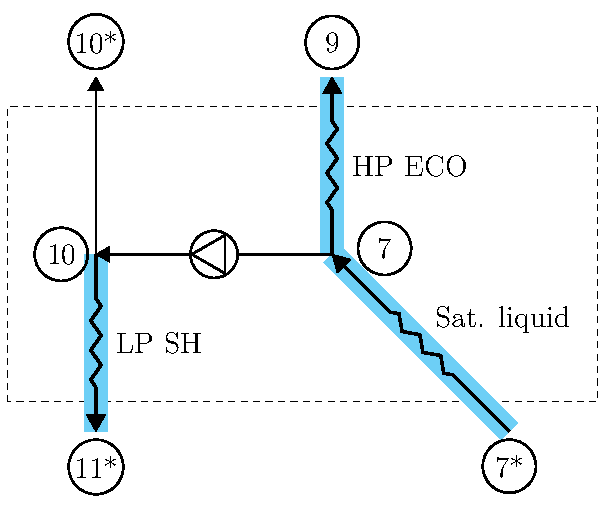
\includegraphics[scale=0.7]{sectionbc_fig.pdf}
    \caption{b-c section flows scheme.}
    \label{fig:sectionbc}
\end{figure}
\begin{figure}[h]
	\centering
    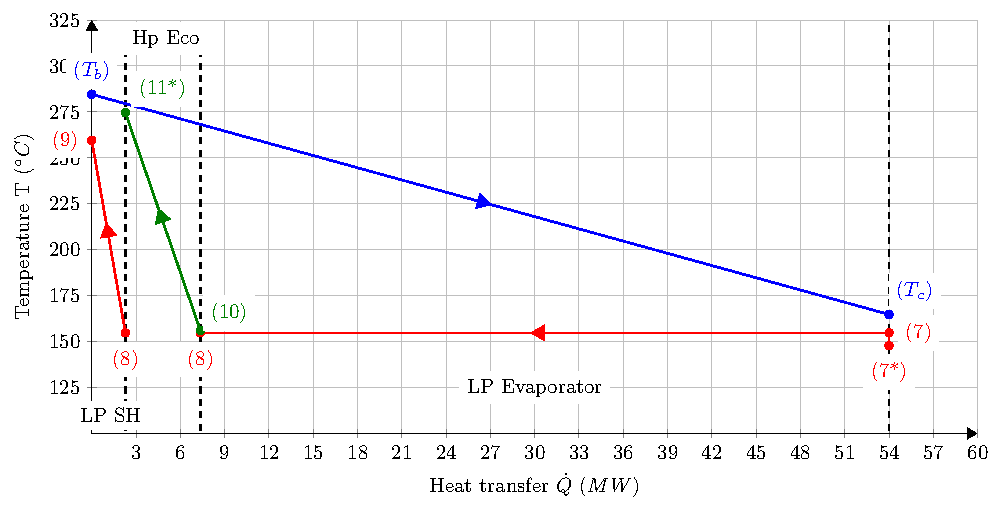
\includegraphics[scale=1]{TQ_plot_LP_fig.pdf}
    \caption{T-Q diagram of b-c section.}
    \label{fig:sectionbc_TQ}
\end{figure}
We make the energy balance in the b-c section of the heat recovery steam generator, paying attention not to consider the contribution given by the HP pump, but only the heat transfer from the flue gases to the steam cycle, like highlighted in cyan in figure \ref{fig:sectionbc}. So the energy balance only refered to the effect of flue gases results:
\begin{equation}
\mdot{FG} \cdot c_{p_{FG}} \cdot (T_b-T_c) \cdot (1-\xi_{HRSG}) = 
\mdotdh{9}{9}{7\first} + \mdotdh{13}{11\first}{10} + \mdotdh{13}{7}{7\first} + \mdotdh{10\first}{7}{7\first}
\label{eq:lp_energy_balance}
\end{equation}
\begin{conditions}
\h{9} & $h(\p{9}, \T{9})$;\\[0.5em]
\p{9} & evaporation pressure in LP section = $5.1\,bar$;\\[0.5em]
\T{9} & $\T{b}-\Delta\T{\text{approach}}$;\\[0.5em]
\h{10} & enthalpy after the feedwater pump;\\[0.5em]
\p{10} & $\frac{\p{evap}^{HP}}{\left( 1- \left. \frac{\Delta p}{p} \right\rvert_{ECO} \right)} $;\\[1.25em]
\h7 & $\h{liq}^{sat}(\p{evap}^{LP})$;\\[0.5em]
\T{c} & $\T{7}^{\text{saturated liquid}}+\Delta\T{\text{pitch point}}$;\\[0.5em]
\end{conditions}
We just miss the enthalpy after the feedwater pump $\h{10}$ that we can evaluate from the definition of hydraulic efficiency of the pump:
\begin{equation}
\label{eq:eta_pump1_iso}
\eta_{hydraulic} \approx \frac{v_7\cdot (\p{10}-\p7)}{\h{10}- \h7} = 75\perc 
\quad \Rightarrow \quad
\h{10} = \h{7} + \frac{\p{10}-\p{7}}{\rho_7 \cdot \eta_{hyd}} = \round{662.190031417057} \kjkg
\end{equation}
In equation \ref{fig:sectionbc} we have two unknowns, $\mdot{9}$ and $\mdot{10\first}$ so we need one more equation to solve it.
We can make energy and mass balance on the manifold from figure \ref{fig:manifold}.
\begin{figure}[H]
	\centering
    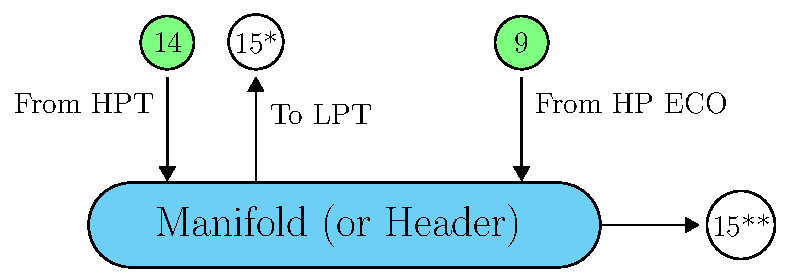
\includegraphics[scale=0.7]{manifold_fig.pdf}
    \caption{Manifold flow scheme.}
    \label{fig:manifold}
\end{figure}
\begin{equation}
\mdoth{9}+\mdoth{14} = \mdoth{9} + \mdot{13}\cdot\h{14} = \mdoth{15\first}+\mdoth{15\doublefirst}
= (\mdot{9}+\mdot{13})\cdot \h{15}
\end{equation}
We have obtained the previous equation noticing that $\mdot{14}=\mdot{13}$ from high pressure turbine mass balance and that $\h{15\first} = \h{15\doublefirst} = \h{15}$ because all the flows going out from a mixing manifold must have the same entropy.

Point 14 is at the outlet of the high pressure turbine, and we know its pressure $\p{14}=5.1\,bar$. From the definition of efficiency of the turbine we can write:

\begin{equation}
\eta_{HPT}^{isoentropic} = \frac{\h{13}-\h{14}}{\h{13}-\h{14}^{IS}} = 84.34\perc
\label{eq:eta_highp_turbine_iso}
\end{equation}
We don't know $\h{14}^{IS}$ but we can compute it from point 13 to point $14^{IS}$ considering an \emph{isoentropic process}:
\[\begin{cases}{}
\p{14}^{IS} = \p{14} = \round{5.1} \,bar \\ 
\s{14}^{IS} = \s{13} = \round{7.041647721675095} \kjkgk
\end{cases}\]
Now we can obtain from \md $\h{14}^{IS} = h(\p{14}^{IS},\s{14}^{IS}) = \round{2.850921794818726e+03} \kjkg$.
\\Reverting equation \ref{eq:eta_highp_turbine_iso} we can get $\h{14}$:
\begin{equation}
\h{14}=\h{13}-\eta_T^{iso} \cdot \left(\h{13} - \h{14}^{IS} \right) = \round{2.955387218744590e+03} \kjkg
\end{equation}

Although we included one more equation we have also added two more unknown, $\mdot{15\doublefirst}$ and $\h{15}$. So we need two more equations that we could get from the energy and the mass balance on the attemperator in figure \ref{fig:attemperator}.
\begin{figure}[H]
	\centering
    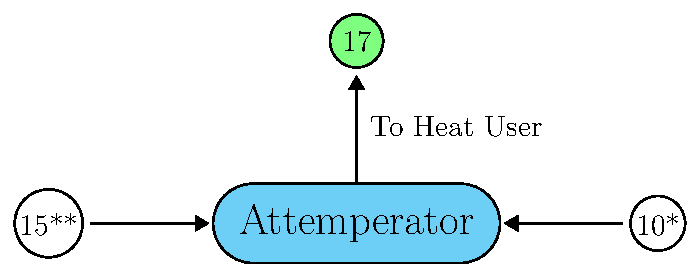
\includegraphics[scale=0.7]{attemperator_fig.pdf}
    \caption{Attemperator flow scheme.}
    \label{fig:attemperator}
\end{figure}
\subparagraph*{Mass balance over Attemperator}
\begin{equation}
\mdot{10\first}+\mdot{15\doublefirst} = \mdot{17} = \round{32.8} \kgs
\end{equation}
\subparagraph*{Energy balance over Attemperator}
\begin{equation}
\mdoth{10\first}+\mdoth{15\doublefirst} = \mdoth{17} = \round{32.8} \kgs \cdot \round{2851.60179874724} \kjkg 
= \round{32.8*2851.60179874724/1000} \mw
\end{equation}
Finally recalling all the four equation we have the non linear system:
\[
\begin{cases}
\Qdot{FG}^{b \rightarrow c} = 
\mdotdh{9}{9}{7\first} + \mdotdh{13}{11\first}{10} + \mdotdh{13}{7}{7\first} + \mdotdh{10\first}{7}{7\first}
\\
\mdoth{9} + \mdot{13}\cdot\h{14} = (\mdot{9}+\mdot{13})\cdot \h{15}
\\
\mdot{10\first}+\mdot{15\doublefirst} = \round{32.8} \kgs
\\
\mdoth{10\first}+\mdoth{15\doublefirst} = \round{32.8*2851.60179874724/1000} \mw
\end{cases}
\]
Solving it with the Broyden method we found the four unknowns:
\[
\begin{bmatrix}
 	\mdot{9}\\
 	\mdot{10\first}\\
	\mdot{15\doublefirst}\\	
	\h{15}
\end{bmatrix} = 
\begin{bmatrix}
	\round{9.94921403932059}\kgs \\
	\round{1.5355631129005}\kgs \\
	\round{31.2644368870995}\kgs \\
	\round{2959.13547865987}\kjkg
\end{bmatrix} \]

\subsection{Condenser}
After the low pressure turbine, the steam flow need to be condensed. We have assumed in point 3 and 4 that we keep from case A to case B the same the heat rejection parameter and the cooling water. So a good way to start is to compute the mass flows and their temperatures around the condenser in plant A.\\ We can write the energy balance at the condenser:
\begin{align}
\Qdot{cond} &= \mdot{w} \cdot c_{p_{w}} \cdot \left(\T{w}^{OUT} - \T{w}^{IN} \right) \\
			&= \mdot{ST} \cdot \left(\h{cond}^{IN} - \h{cond}^{OUT} \right) \\
			&= U \cdot A \cdot \Delta\T{\text{mean log}}
\end{align}
\begin{conditions}
\h{cond}^{IN}  & the enthalpy of the steam at the outlet of the low pressure turbine;\\[0.5em]
\h{cond}^{OUT} & is the enthalpy of saturated liquid at $\p{cond}$;\\[0.5em]
\end{conditions}
So we can get the last unknown $\mdot{w}$ reverting the equation:
\begin{equation}
\mdot{w} = \frac{\mdot{ST} \cdot \left(\h{cond}^{IN} - \h{cond}^{OUT} \right) }
 				{c_{p_{w}} \cdot \left(\T{w}^{OUT} - \T{w}^{IN} \right)}
 		 = \round{1.636331926175822e+03} \kgs
 		 = \round{1.636331926175822e+03/1000} \mcubes
\end{equation}
Now we must procede with the same balance in plant B. In this case howether we miss the condensation pressure of the steam cycle so we cannot use the mean log method. So we must apply the NTU approach. For any heat exchanger it is valid that the effectiveness $\varepsilon$ is:
\begin{equation}
\varepsilon = f\left(NTU, \frac{C_{min}}{C_{max}} \right) 
\label{eq:effectiveness_1}
\end{equation}
\begin{conditions}
C_i  & $\mdot{i} \cdot c_i$ is the heat capacity;\\[0.5em]
NTU  & $\frac{UA}{C_{min}}$ is the number of transfer units.
\end{conditions}
Since $\left.U \cdot A \right|_A = \left.U \cdot A \right|_B$ for hypothesis and the minimum heat capacity is on the side of cooling water 
\footnote{The steam does not change its temperature in the condenser so $C_{ST} = \frac{\Qdot{} \neq 0}{\Delta T = 0} \rightarrow 				\infty$} 
and for the two cases is approximately the same 
\footnote{$c_p$ of water used is a mean value and it can change a bit since we don't know at this point the outlet temperature of 				the water at the outlet of the condenser.}
and the ratio $C_{min}/C_{max}$ in both plants tents to zero we can assert that also the effectiveness that is function of NTU and $\frac{C_{min}}{C_{max}}$ is the same. $\varepsilon$ is also evaluable as the condensation heat transfered over the maximum heat transferable or in formulas:
\begin{equation}
\varepsilon = \frac{\Qdot{cond}}{\Qdot{MAX}} 
= \frac{ \cancel{C_{w}} \cdot \left(\T{w}^{OUT} - \T{w}^{IN} \right)}
	   { \cancel{C_{w}} \cdot \left(\T{steam}^{IN} - \T{w}^{IN} \right)}
\label{eq:effectiveness_2}
\end{equation}
But $\varepsilon_A = \varepsilon_B$ and we can easily compute $\varepsilon_A$ since we know both inlet and outlet temperature of the cooling water and the condensation temperature corresponding to $\p{cond} = 0.08\,bar$. 
\begin{equation}
\varepsilon_A = \frac{ \cancel{C_{w}} \cdot \left(\T{w}^{OUT} - \T{w}^{IN} \right)}
	   { \cancel{C_{w}} \cdot \left(\T{steam}^{IN} - \T{w}^{IN} \right)} 
= \round[round-precision=3]{0.464898907511811}
= \varepsilon_B
\label{eq:effectiveness_A}
\end{equation} 
We can write the energy balance at the condenser of re-powering plant:
\begin{align}
\Qdot{cond} &= \mdot{w} \cdot c_{p_{w}} \cdot \left(\T{w}^{OUT} - \T{w}^{IN} \right) \\
			&= \mdot{ST} \cdot \left(\h{cond}^{IN} - \h{cond}^{OUT} \right) 
			 = \mdot{16} \cdot \left(\h{16} - \h{1} \right) 
			\label{eq:condenser_balance_steam_side}
\end{align}
$\T{w}^{OUT}$ can be obtained from equation \ref{eq:effectiveness_A}:
\begin{equation}
\T{w}^{OUT} = \T{w}^{IN} + \varepsilon_A \cdot \left(\T{steam}^{IN} - \T{w}^{IN}  \right)
\end{equation}
\begin{conditions}
\T{w}^{IN}  	& $20 \celsius$;\\[0.5em]
\T{steam}^{IN}  & $\T{16} = \T{sat}(\p{cond}) = f(\p{cond})$.
\end{conditions}
So $\T{w}^{OUT}$ is a function only of $\p{cond}$.
Now we have express every term in water side of energy balance at the condenser as a function of just one unknown but all the quantities in equation \ref{eq:condenser_balance_steam_side} are unknown. 
\\With the mass balance on the manifold we can get $\mdot{16} = \mdot{15x}$:
\begin{equation}
\mdot{16} = \mdot{15x} = \mdot{13} + \mdot{9} - \mdot{15xx} = \round{35.6679293583318} \kgs
\end{equation}

Point 1, at the outlet of the condenser, is saturated liquid at the condensation pressure so we can get the value of its enthalpy from \md of saturated liquid:
\begin{equation}
\h1 = \h{liq}^{sat}(\p1) = \h{liq}^{sat}(\p{cond}) = f(\p{cond}).
\end{equation} 

Point 16 is at the outlet of the low pressure turbine, and its pressure is our main unknown $\p{cond}$. From the definition of efficiency of the turbine we can write:
\begin{equation}
\eta_{LPT}^{isoentropic} = \frac{\h{15\first}-\h{16}}{\h{15\first}-\h{16}^{IS}} = 87.55\perc
\label{eq:eta_lp_turbine_iso}
\end{equation}
We don't know $\h{16}^{IS}$ but we can compute it from point $15\first$ to point $16^{IS}$ considering an \emph{isoentropic process}:
\[\begin{cases}{}
\p{16}^{IS} = \p{16} = \p{cond} \\ 
\s{16}^{IS} = \s{15\first} = \round{7.277892496559714} \kjkgk
\end{cases}\]
Now we can obtain from \md $\h{16}^{IS} = h(\p{16}^{IS},\s{16}^{IS}) = f(\p{cond})$.
\\Reverting equation \ref{eq:eta_lp_turbine_iso} we can get $\h{16}$:
\begin{equation}
\h{16}=\h{15\first}-\eta_T^{iso} \cdot \left(\h{15\first} - \h{16}^{IS} \right) = f(\p{cond})
\end{equation}
So the balance becomes:
\begin{equation}
\mdot{w} \cdot c_{p_{w}} \cdot \left(\T{w}^{OUT}(\p{cond}) - \T{w}^{IN} \right)
= \mdot{16} \cdot \left(\h{16}(\p{cond}) - \h{1}(\p{cond}) \right) 
\end{equation}
We can solve the non-linear equation in the same way we solve equation \ref{eq:hp_energy_balance}, with secants method and we obtain $\p{cond} = \round[round-precision=3]{0.0938399542235199}\,bar$.

The thermodynamical properties at the inlet and the outlet of the condenser are in table \ref{table:point_condenser}.
\begin{table}[h]
\centering
\caption{Thermodynamical properties at the condenser.}
\label{table:point_condenser}
\begin{tabular}{@{}lcccc@{}}
\toprule
Condenser & p                               & T                           & h                                	& $\chi$ \\ \midrule
Inlet     & $\round{0.0938399542235199}\,bar$  & $\round{44.5694817842618}\celsius$ & $\round{2.380186424505560e+03}\kjkg$ & $\round{0.915867706000774}$
\\
Outlet    & $\round{0.093839954223520}\,bar$ & $\round{44.569481784261825}\celsius$              & $\round{1.866378690849691e+02}\kjkg$ & 0 \\ \bottomrule
\end{tabular}
\end{table}

\subsection{Performances}
To evaluate the performances of the re-powered combined cycle we need to evaluate the power produced and consumed by every turbomachine, pump or turbine. For simplicity we consider the mechanical and \emph{electrical efficiency}  of the pumps and the turbines only at the end of the calculations.

\subsubsection*{Pump after condenser}
\begin{equation}
\Wdot{pump}^{1-2} = \mdotdh{1}{2}{1} = \mdotdh{16}{2}{\text{cond out}}
\end{equation}
We do not directly have the enthalpy $h_2$ but we can obtain it from the definition of efficiency of the pump:
\begin{equation}
\label{eq:eta_pump12_iso}
\eta^{pump}_{hyd} = \frac{h_2^{IS}-h_1}{h_2-h_1} = 75\perc
\end{equation}
We can estimate $h_2^{IS}-h_1 \approx \frac{p_2-p_1}{\rho_1}$ with hypothesis of \emph{incompressible flow} and \emph{density constant} with temperature and pressure. So reverting equation \ref{eq:eta_pump12_iso} we get:
\begin{equation}
h_2 = h_1 + \frac{p_2-p_1}{\rho_1 \cdot \eta_{hyd}} = \round{186.761617054565} \kjkg
\end{equation}
So finally we obtain $\Wdot{pump}^{1-2} = \round{4.41383383779206} \kw $

\subsubsection*{Pump low pressure}
\begin{equation}
\Wdot{pump}^{6-5} = \mdotdh{5}{6}{5}
\end{equation}
\begin{figure}[h]
	\centering
    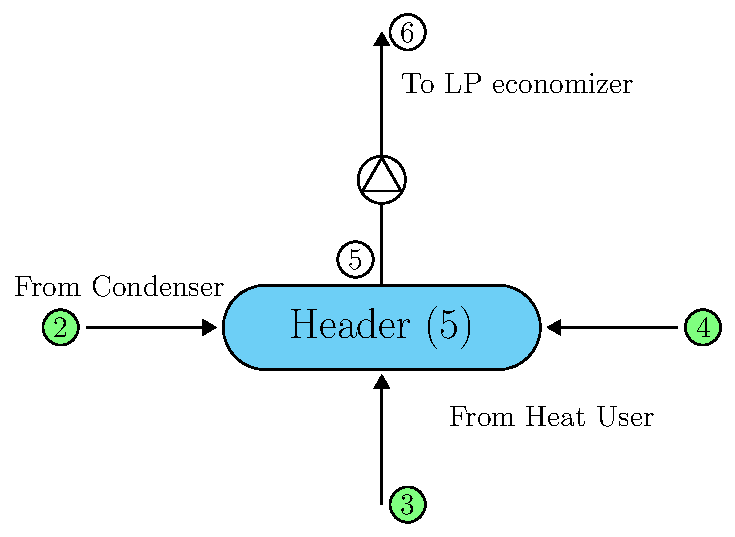
\includegraphics[scale=0.7]{header5_fig.pdf}
    \caption{Mixer flow scheme.}
    \label{fig:header5}
\end{figure}
From mass end energy balance of the header in figure \ref{fig:header5} we obtain $\mdot{5}$ and $\h{5}$:
\begin{equation}
\mdot{5} = \mdot{1} + \mdot{user1} + \mdot{user2} = \round{68.4679293583318} \kgs 
\end{equation}
\begin{equation}
\mdoth{5} = \mdoth{1} + \mdoth{user1} + \mdoth{user2} 
\quad \Rightarrow \quad
\h{5} = \round{240.755862455804} \kjkg 
\end{equation}
We do not directly have the enthalpy $h_6$ but we can obtain it in the same way as pump between points 1 and 2 with the definition of efficiency of the pump:
\begin{equation}
h_6 = h_5 + \frac{p_6-p_5}{\rho_5 \cdot \eta_{hyd}} = \round{241.309388560126} \kjkg
\end{equation}
So finally we obtain $\Wdot{pump}^{5-6} = \round{37.8987862086979} \kw $

\subsubsection*{Pump high pressure}
\begin{equation}
\Wdot{pump}^{7-10} = \mdotdh{7}{10}{7} = \left( \mdot{10\first} + \mdot{11\first} \right) \cdot \left( \h{10} - \h{7} \right)
\end{equation}
We have already calculated $\h{10}=\round{6.621900314170566e+02}\kjkg$ and $\h{7}=\round{6.528294517961159e+02}\kjkg$ in low pressure section. So the power required by the pump is $\Wdot{pump}^{7-10} = \round{547.769094058767} \kw $


\subsubsection*{High pressure turbine}
\begin{equation}
\Wdot{turbine}^{HP} = \mdotdh{13}{13}{14}
\end{equation}
We have already calculated 
$\mdot{13}=\round{56.983152206110724}\kgs$, 
$\h{13}=\round{3.518006238789766e+03}\kjkg$ and 
$\h{14}=\round{2.955387218744590e+03}\kjkg$ in high pressure section. So the power produced by the turbine is $\Wdot{turbine}^{HP} = \round{32059.8052532871/1000} \mw $

\subsubsection*{Low pressure turbine}
\begin{equation}
\Wdot{turbine}^{LP} = \mdotdh{15\first}{15\first}{16}
\end{equation}
We have already calculated 
$\mdot{15\first}=\round{35.6679293583318}\kgs$, 
$\h{16}=\round{2380.18642450556}\kjkg$ and 
$\h{15\first}=\round{2959.13547865987}\kjkg$ in high pressure section. So the power produced by the turbine is $\Wdot{turbine}^{LP} = \round{32059.8052532871/1000} \mw $
\\ \\
The net electric power of the plant B is equal to:
\begin{equation}
\Wdot{net} = \Wdot{GT} + \eta_m \cdot \eta_e \cdot \Wdot{turbines} - \frac{\Wdot{pumps}}{\eta_{m/e}} - \Wdot{auxiliares} 
= \round{190429.335293953/1000} \mw 
\end{equation}
\\
The fuel power of the gas turbine is equal to:
\begin{equation}
\Qfuel = \frac{\Wdot{GT}}{\eta_{GT}} 
= \round{411594.202898551/1000} \mw 
\end{equation}
\\
The heat user power is equal to the user in plant A:
\begin{equation}
\dot{Q}_B = \dot{Q}_A
= \round{83709.8837796313/1000} \mw 
\end{equation}
\\
Finally with all the power exchanged in the plant we can evaluate all the performance parameters:
\begin{itemize}
\item Electric net efficiency $\displaystyle \eta_{el} = \frac{\Wel}{\Qfuel} = \round{0.462662821664889*100}\perc$.
\item Thermal net efficiency $\displaystyle \eta_{th} = \frac{\Qth}{\Qfuel} = \round{0.203379647211076*100}\perc$.
\item Total net efficiency $\displaystyle \eta_{I} = \eta_{el} + \eta_{th} = \frac{\Wel+\Qth}{\Qfuel} = \round{0.666042468875965*100}\perc$.
\item Primary energy saving $\displaystyle PES = 1-\frac{\Qfuel}{\Wel/\eta^{REF}_{el}  +  \Qth/\eta^{REF}_{th}}
 = {\round[round-precision=3]{0.096853358456945}>0}$.
\end{itemize}

With the repowering we have obtained a \emph{positive} primary energy saving index so it is convenient to repower plant A to a new combined cycle feeded by a gas turbine.

\end{document}

